\chapter{Validation of the \ke\, model} % (fold)
\label{cha:validation_of_k_epsilon_model}

In the following section, the results of simulations with the Chien-wall-model are shown. These results were compared with the results of the algebraic turbulence model, which were created for worksheet 2, and with literature. Also the choice of the wall model was investigated.

\section{Channel flow} % (fold)
\label{sec:channel_flow}

Different cases of channel flow were performed under following conditions:

\begin{center}
\begin{tabular}{lccc}
\hline 
Re        & 1000 & 5600 & 13750\\\hline         
Uniform velocity profile $u$         & \multicolumn{3}{c}{1.0}\\
Geometry  & \multicolumn{3}{c}{100\,$\times$\,1} \\
Mesh type & \multicolumn{3}{c}{uniform} \\
Mesh      & 64\,$\times$\,128 & 64\,$\times$\,256 & 64\,$\times$\,512 \\\hline 
\end{tabular}
\end{center}


\subsubsection*{Velocities}
Figure~\ref{fig:channel-u-profile} shows the u-velocity component along the cross section for a laminar simulation, an algebraic simulation and a $k$-$\epsilon$\,simulation (both for Re$=5600$). The position of measurement and time were adjusted according to the case, so that the flow profile was stationary and fully developed.

\begin{figure}[!htb]
\centering
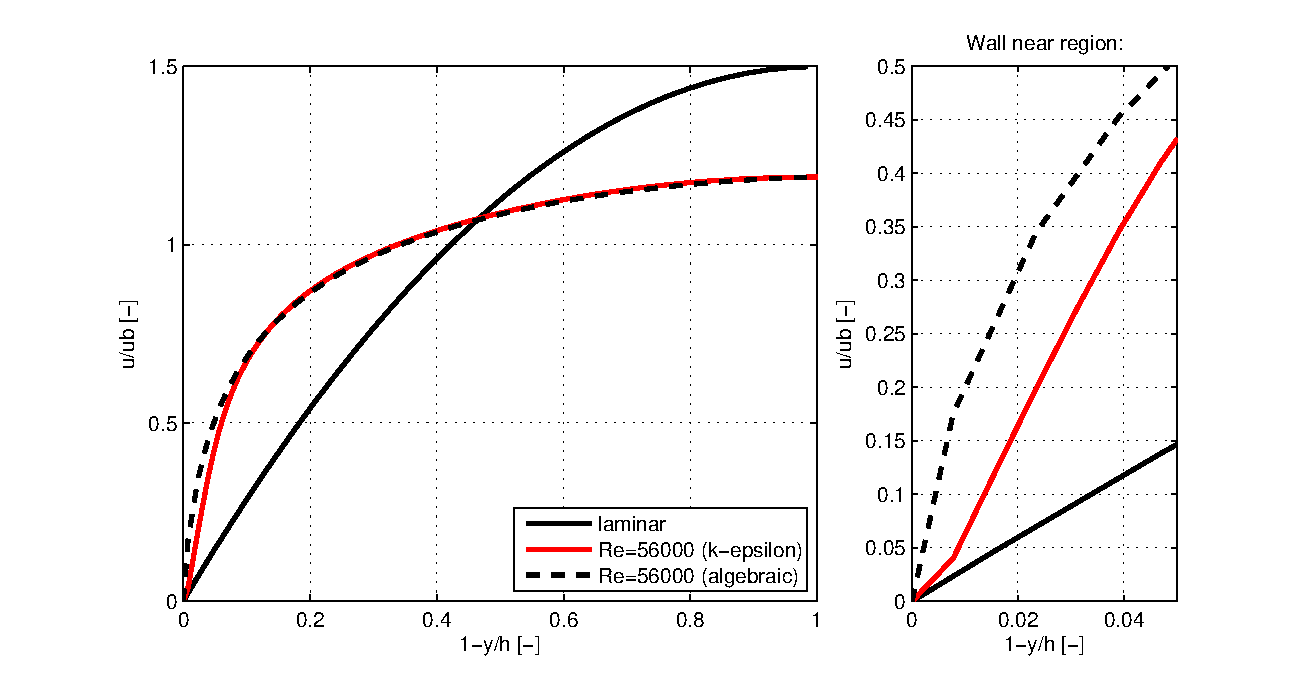
\includegraphics[width=1.0\textwidth]{FIGURES/vprofile.eps}
\caption{u-velocity profile}
\label{fig:channel-u-profile}
\end{figure} 


\noii The velocities behave as expected. In the laminar case, the velocity profile has a parabolic form with a maximum of 1.5m/s. The turbulent simulations result in lower maximum velocities (u $\le$ 1.5m/s) and in a higher slope of the velocities near the wall: the results for both turbulent models are comparable (for a more detailed comparison see the following sections).

\newpage
\subsubsection*{Shear stress}

Figure~\ref{fig:channel-tau} shows the shear stress profile along the cross section for each turbulent case. The shear stress components are normalized with $\tau_{net}=\tau_v+\tau_r$:

\begin{itemize}
\item viscous stress $\tau_v=\rho\nu\abl{\ave u}{y}$
\item Reynolds stress $\tau_r=-\rho\ave{u' v'}=\rho\nu_t\abl{\ave u}{y}$
\end{itemize}

\begin{figure}[!htb]
\centering
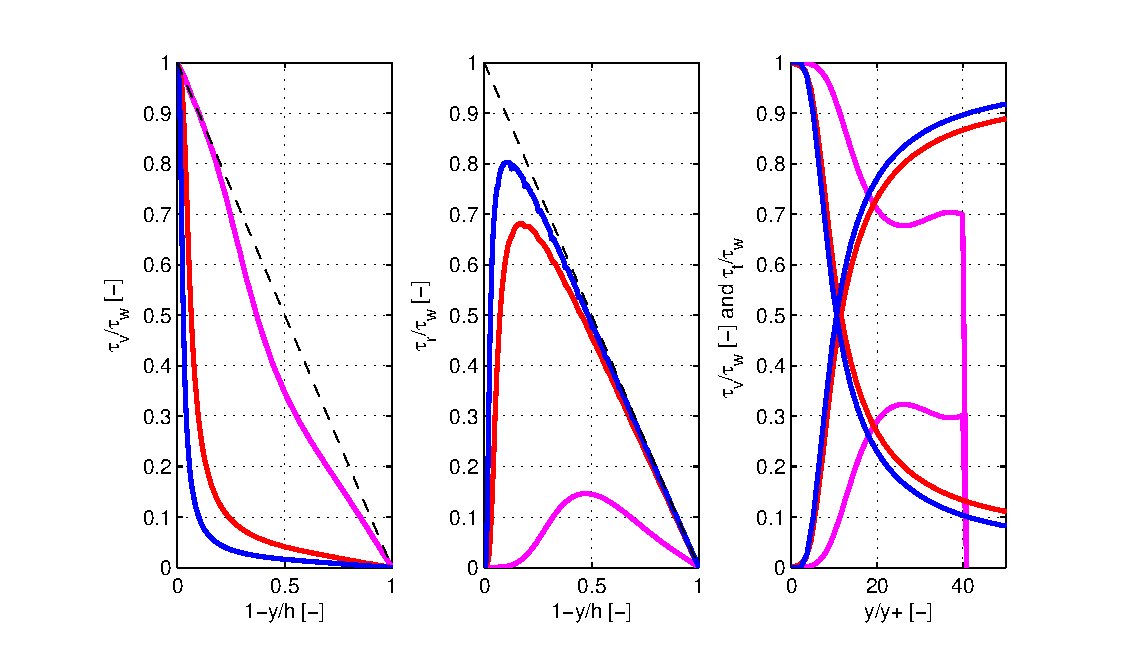
\includegraphics[width=1.0\textwidth]{FIGURES/tau.eps}
\caption{Shear stresses (viscous stress and Reynolds stress - for legend see next figure)}
\label{fig:channel-tau}
\end{figure} 

\noindent Additionally, the shear stress components are plotted over $y^+$. Self-similarity is clearly recognisable.


\newpage
\subsubsection*{Comparison with the literature: velocity profile for Re=5600}\label{ssub:litkim}
Following additional values have been estimated for the turbulent Re=5600 case:
\begin{align}
u_\tau=\sqrt{\tau_w/\rho}
\qquad\qquad
l^+=\nu/u_\tau
\qquad\qquad
Re_\tau=u_\tau\cdot\delta/\nu
\end{align}
Dimensionless dimensions were created with these values and were compared with the measurement values from the literature \citep{kim1987}.

\begin{center}
\begin{tabular}{lccc}
\hline
 & Literature & Algebraic & $k$-$\varepsilon$ \\\hline
$Re_\tau$ & 180 & 352 & 170 \\
$Re_c$ & 3300 & 3329 &  3329 \\
$Re_m$ & 5600 & 5600 & 5600 \\
$u_m/u_\tau$ & 15.63 & 7.95 & 16.48 \\
$u_c/u_\tau$ & 18.20 & 9.45 & 19.59 \\
$u_c/u_m$ & 1.16 & 1.189 & 1.189 \\
$C_f = \tau_w / (0.5 \rho u_m^2)$ & 8.18$\times$10$^{-3}$ & 31.6$\times$10$^{-3}$ & 7.37$\times$10$^{-3}$ \\\hline
\end{tabular}
\end{center}

\noindent The simulated maximal velocity $u_c/u_m$ matches well with the value from the literature for both turbulent simulations. The $k$-$\epsilon$ model estimates all the $\tau_w$-related variables ($Re_\tau$, $C_f$, $u_\tau$...) much more precisely. In our last report \citep{lienen2015} we discussed, that $\tau_w$  is overestimated by the more simple model, which implies that the wall near slope of x-component of the velocity is too high.

\subsubsection*{Sublayers}\label{ssub:sublayers}

Figure~\ref{fig:sublayers_y+}-left shows the normalized velocity $w^+$  over $y^+$ and the expected velocity profile. They do match very well for high Reynolds-numbers: the linear sublayer is described exactly, the logarithmic layer shows slight discrepancy from the expectations.

\begin{figure}[!htb]
\centering
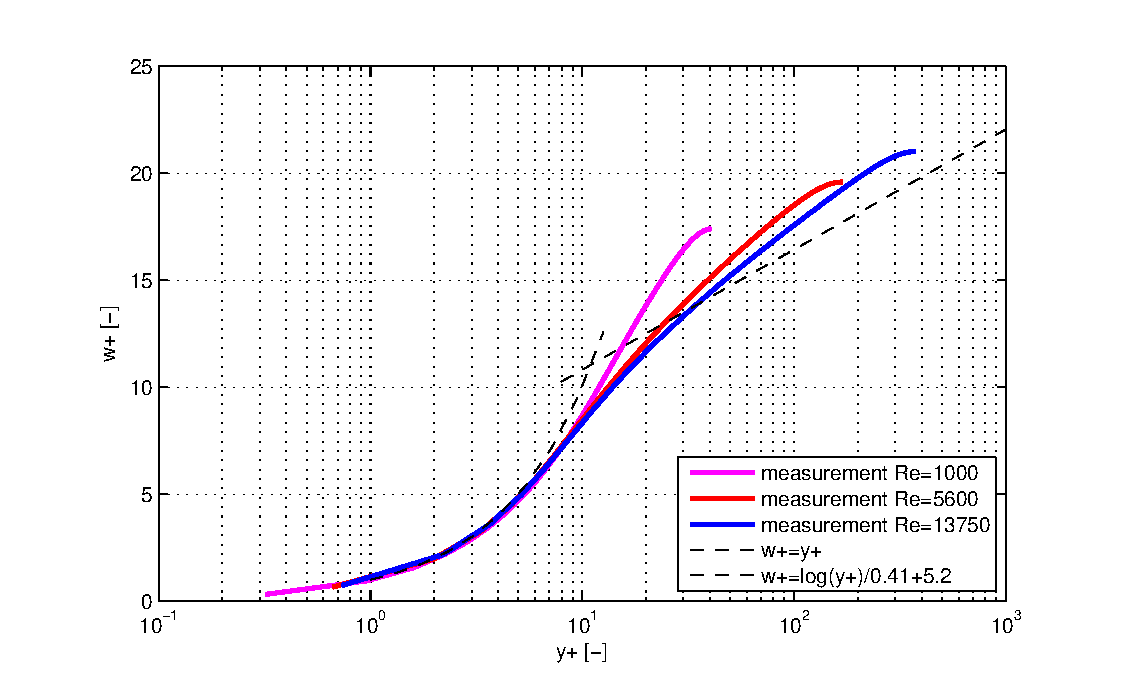
\includegraphics[trim=35 0 30 0,clip,width=0.49\textwidth]{FIGURES/wplusyplus.eps}
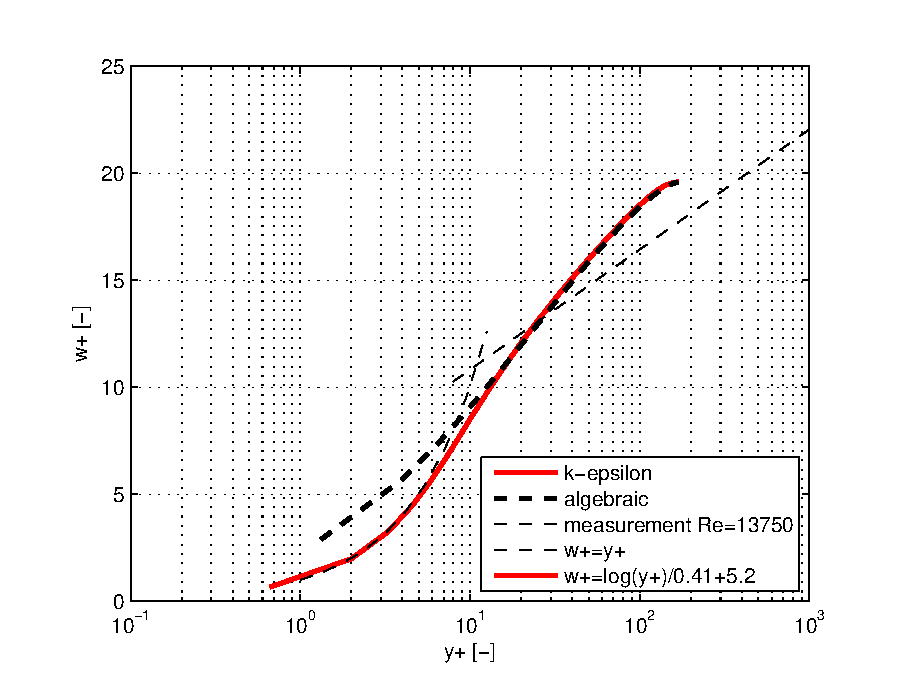
\includegraphics[trim=35 0 30 0,clip,width=0.49\textwidth]{FIGURES/avske.eps}
\caption{Sublayers: $w^+$ over $y^+$ (left: \ke\, with Re=1000, =5600 and =13750; right: Re=5600 with \ke\, and algebraic turbulence model)}
\label{fig:sublayers_y+}
\end{figure} 

\noindent Figure~\ref{fig:sublayers_y+}-right also shows a modified normalized velocity $w^+$ over $y^+$ for the algebraic turbulence model for Re=5600. In this case, $l^+$ and $u_{\tau}$ were calculated with the $\tau_w$-value estimated with the help of the \ke\, simulation: the results correspond well in the logarithmic sublayer, not that well in the linear sublayer. As expected, the slope of the velocity is too high near the wall for the algebraic model.

\newpage
\subsubsection*{Comparison with the literature: TKE profile for Re=13750}

In the following, the single terms in the $k$-transport equation are examined in more detail. The implemented form of this equation has the following form:

\begin{align}
\abl{k}{t} + u_i\,\abl{k}{x_i}
&=
\abl{}{x_i}\left(  B_k \abl{k}{x_i} \right) 
-
f_3\,\frac{1}{T} \, k
+
F
-
D
\end{align}
For a stationary fully developed channel flow, the equation reduces to the following form:
\begin{align}
0
&=
\underbrace{
\abl{}{y}\left(  B_k \abl{k}{y} \right) 
}_{1}
\underbrace{
-
f_3\,\frac{1}{T} \, k
-
D
}_{2}
\underbrace{+
F}_3
\end{align}
with the diffusion term (1), the dissipation term (2) and the production term (3) being in equilibrium. Figure~\ref{fig:pop_tke} shows the profile of each term in the wall near region ($y^+<50$).
\begin{figure}[!htb]
\centering
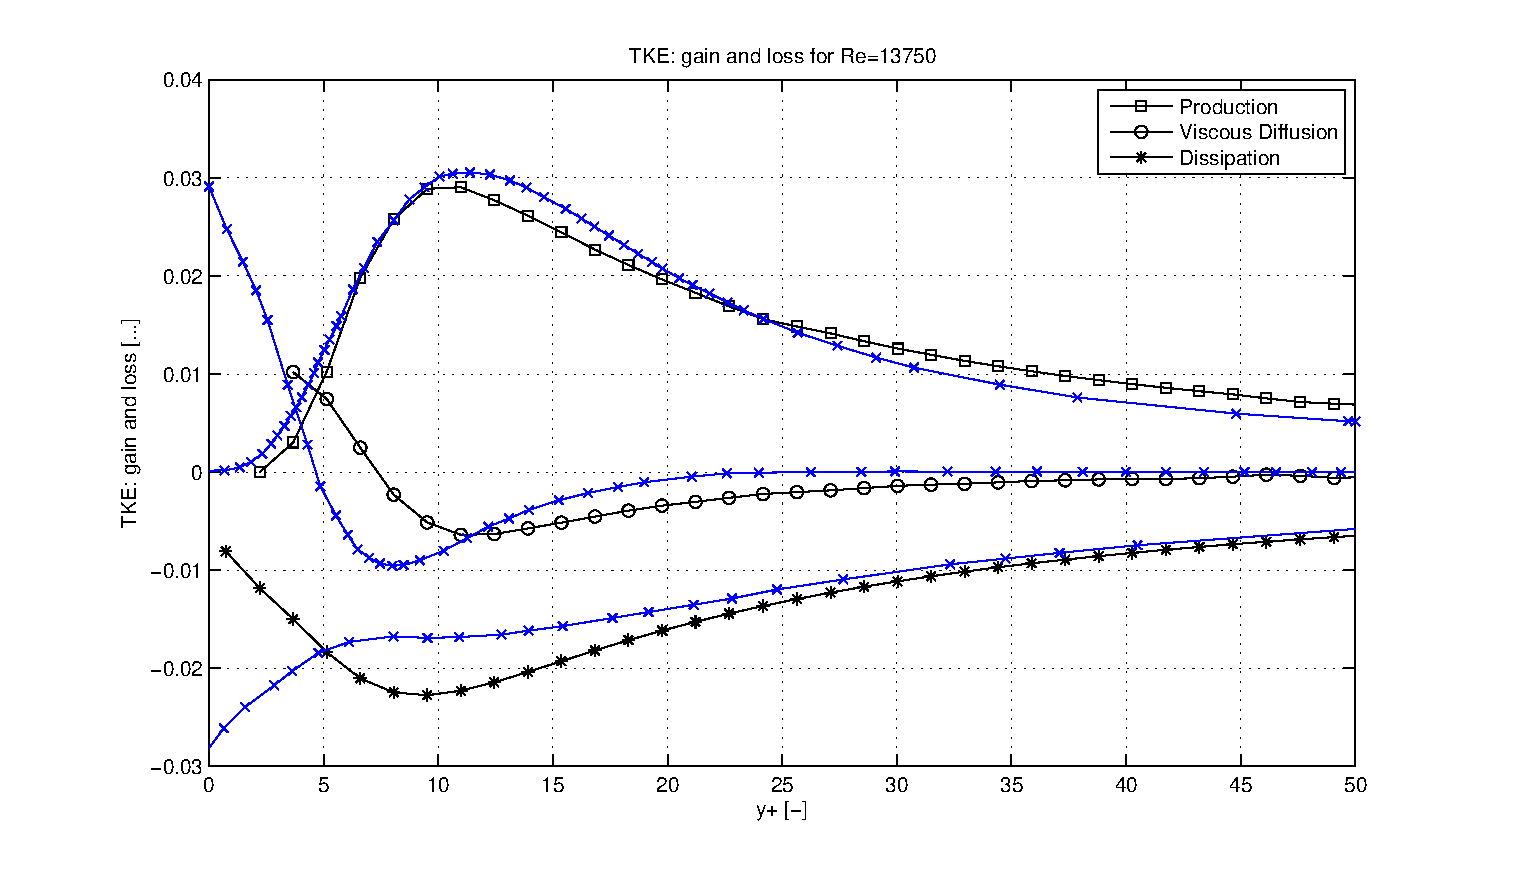
\includegraphics[trim=60 20 60 15,clip,width=0.95\textwidth]{FIGURES/tkegainloss.eps}
\caption{Terms of the TKE-transport equation for Re=13750 (in comparison with the literature \citep{pope2000} p. 285, scaled by 0.13)}
\label{fig:pop_tke}
\end{figure} 

\noii The production increases from zero at the wall and reaches its peak value well within the buffer layer, at $y^+=10$ (Pope: $y^+=12$). Around this peak, production exceeds dissipation by a factor of 1.4 (Pope: 1.8) and the excess energy produced is transported away by viscous diffusion to the wall. The dissipation is balanced by viscous transport. The peak dissipation should occur at the wall, but it does not. In the simulation, the locations of the maximal production and of the dissipation coincide.


\subsubsection*{Influence wall model}

In the case that no wall model is used during the \ke\,simulation, the profile of each term of the $k$-transport equation looks completely different. The maximum production and dissipation are at the wall. The excess energy production is transported away from the wall.

\begin{figure}[!htb]
\centering
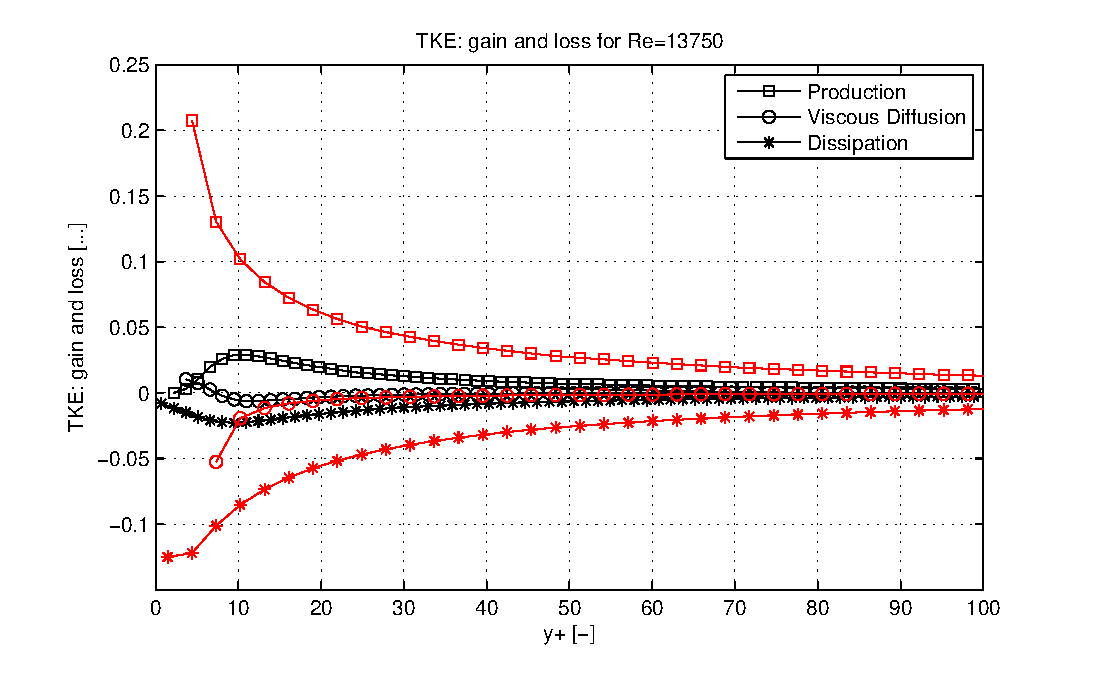
\includegraphics[width=0.95\textwidth]{FIGURES/nowallmodel.eps}
\caption{Terms of the TKE-transport equation for Re=13750 (red: without wall model; black: Chien)}
\label{fig:reswithoutwallmodel}
\end{figure} 

% subsection channel_flow (end)

\newpage
\section{Boundary layer} % (fold)
\label{sec:boundary_layer}



To further validate the implemented flow models, boundary layer simulations were performed for the laminar case and the \textit{k}-$\varepsilon$ turbulence model. The influence of wall models on the \textit{k}-$\varepsilon$ model was considered as well. The final results were compared to theoretical values.

\noii To start with, theoretical solutions for the boundary layer, over a flat plate without pressure gradient are presented. For a laminar flow and the before mentioned assumptions, an analytical solution for the boundary layer equations according to Blasius exists. It states for the boundary layer thickness
\begin{equation}
	\delta_{laminar} \approx 3.5\,\sqrt{\frac{2\nu x}{U_\infty}} = 3.5\,\sqrt{\frac{2x}{Re\,U_\infty}}.
\end{equation}
For a turbulent flow and the same assumptions the boundary layer thickness is given by
\begin{equation}
	\delta_{turbulent} \approx 0.16\,x / Re_x^{1/7},
\end{equation}
according to \citep{stemmer2015}.
Therein, the Reynolds number $Re_x$ can be calculated by
\begin{equation}
	Re_x = \frac{U_\infty x}{\nu} = U_\infty\,Re\,x.
\end{equation}
A second theoretical formula to determine the turbulent boundary layer thickness can be found in worksheet 2 of this HPC lab and states
\begin{equation}
	\delta_{turbulent} \approx 0.382\,x/Re_x^{1/5}.
\end{equation}
The simulation was performed for a plate of length $25$ and height $1$. A uniform inlet velocity profile with $U_\infty = 1.0$ was chosen. The domain was discretized by $128\times256$ cells in x- respectively y-direction. The simulation was performed for $Re=13750$. 
Furthermore, the final simulation time was chosen so that a quasi steady flow had developed. The results are shown in figure~\ref{fig:boundarylayerthickness}.

\begin{figure}[!htb]
\centering
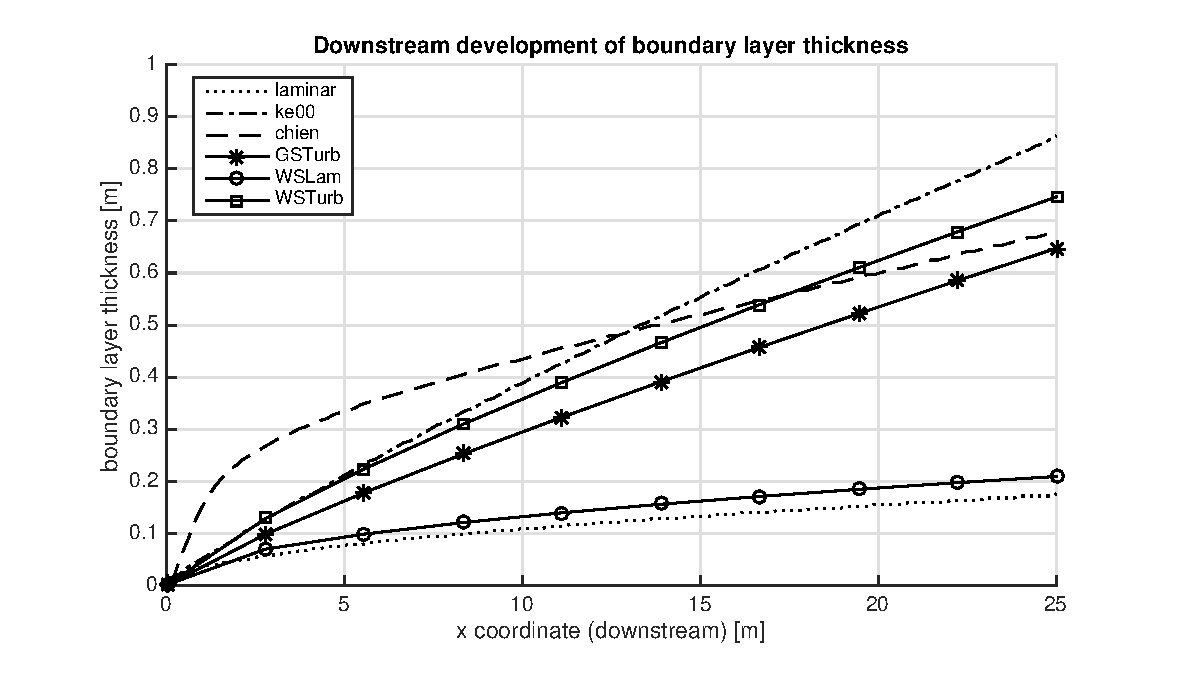
\includegraphics[width=0.78\textwidth]{FIGURES/blThickness.eps}
\caption{Boundary layer thickness over x}
\label{fig:boundarylayerthickness}
\end{figure} 


\begin{figure}[!htb]
\centering
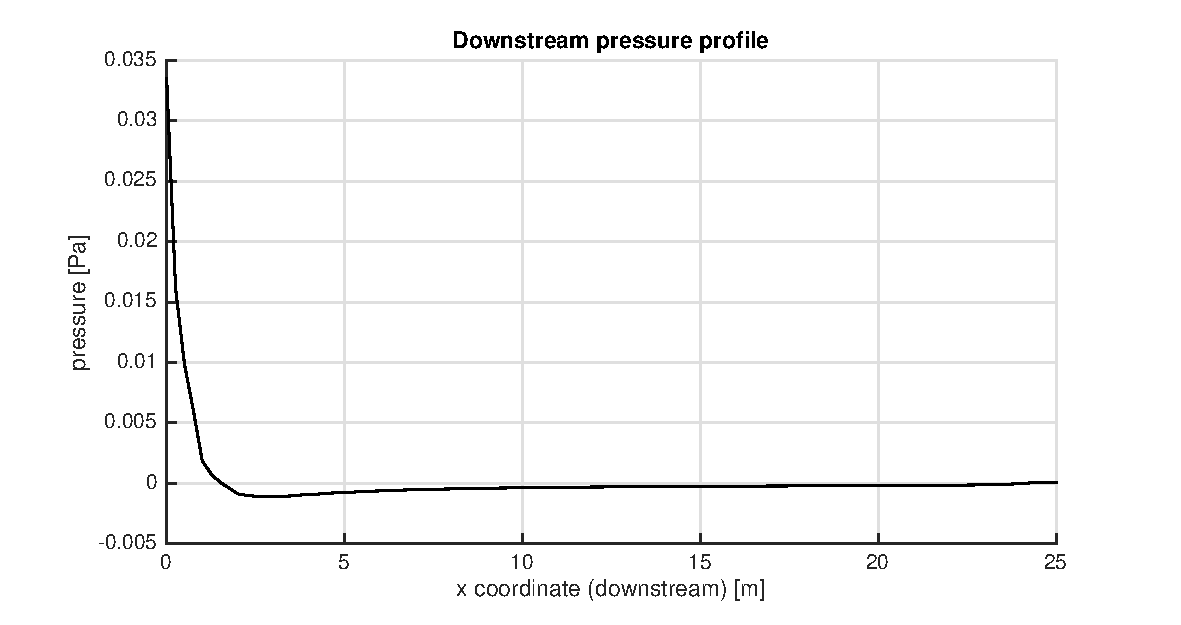
\includegraphics[width=0.78\textwidth]{FIGURES/pressure.eps}
\caption{Pressure profile at the height of $y=0.1m$}
\label{fig:boundarylayerpressure}
\end{figure} 

\noii In addition, figure~\ref{fig:boundarylayerpressure} shows exemplarily the pressure field at the last timestep for the laminar simulation. The pressure fields for both turbulent simulations are similar and are thus not shown here. Some distance behind the inlet, the pressure is nearly constant as can be seen easily. Due to that, the constant pressure assumptions made for the theoretical equations nearly match the simulation.

\noii Comparing the overall spatial developing of the boundary layer thickness of the laminar and the turbulent simulations, their boundary layer thickness profile behaves as expected. The laminar boundary layer is thinner than in turbulent cases. In addition, some distance behind the inlet the \textit{k}-$\varepsilon$ simulation without a wall model results in a thicker boundary layer. This is due to the fact, that for this model the turbulent viscosity $\nu_T$ is not damped near the wall, and thus the wall normal momentum transport is also not damped compared to Chiens model. Near the inlet, this behaviour can not be detected. Presumably this is due to the influence of the inlet boundary conditions.

\noii The laminar simulation yields pretty good results when comparing to the Blasius solution. They match except for a scaling factor. For the turbulent simulations, the results deviate from the theoretical values of about $20\%$. Furthermore, the results without wall function tend to match the profile better.

\noii As expected, no transition between laminar and turbulent boundary layer could be encountered.

% subsection boundary_layer (end)

% chapter validation_of_k_epsilon_model (end)